\begin{abstract}
 The abstract goes here... (BITCOIN influence -> Blockchain). Captivate readers attention.
\end{abstract}




%*****************************************
\chapter{Introduction}
%*****************************************

Blockchain (BC) has been considered as one of the most promising disruptive technologies during the last years. Many market-leading companies, experts and global innovators have referred it as the "Next Generation of the Internet" \cite{JenClarck2017}, succeeding the World Wide Web era. Evaluating its potential benefits, different banks and major enterprises, such as UBS, Microsoft or IBM, have already accomplished important investments in such innovative technologies.

The revolution started in 2008, with a whitepaper publication by Satoshi Nakamoto \cite{nakamoto2008bitcoin}, who introduces a new digital payment protocol called Bitcoin. Satoshi Nakamoto is just a name used by an unknown person or group of people to first reference the implementation. Nowadays, Bitcoin's creator still remains a mystery.

In 2009, a deployed software version based on the paper was launched. Bitcoin uses an alternative virtual currency, to make trusted transactions between different peers. This system relies on a distributed database allocated on the Internet, the blockchain. Blockchain uses a peer-to-peer architecture model combined with secure protocols, such as public key cryptography, which intentionally removes the presence of middle-parties or intermediaries. Thus, in the case of Bitcoin, it eliminates the main party for transactions: central banks.

At the beginning, the blockchain architecture was restricted to only one application: online payments. However, after observing its advantages and possible use cases, an improvement of Bitcoin emerged: Ethereum \footnote{\url{https://www.ethereum.org/}}. By contrast, Ethereum extends the power of decentralized transactions with a Turing-complete contract system. A Turing-complete system can perform any computation, with just writing a few lines of code, which then creates a smart contract. A smart contract can be written with non-restrictive and user-friendly programming languages, allowing developers to easily learn and benefit from them. Therefore, it brings to the user the opportunity to develop their own applications. Smart contracts applications are called decentralized apps, and unlike normal web apps, they may not be allocated in a central server. In other words, they use blockchain technology to retrieve and store data instead of a database.


\section{Motivation}

Nowadays, blockchain is becoming a trending topic in the business world. Thousands of articles, research papers and books, such as: How the technology behind bitcoin is changing money, business and the world \cite{tapscott2016blockchain} or Blockchain: Blue print for a new economy \cite{swan2015blockchain}, are catching the public eye. Nevertheless, as it is an emerging technology, a necessity to look towards new horizons exists. Through the above mentioned Ethereum smart contracts, this task will be easier to handle and manage, which opens up new possibilities to approach existing problems. Hence, blockchain technology can be used in many applications beyond currency.

Many use cases are currently derived from blockchain, e.g: candidate's voting or asset tracking \cite{abeyratne2016blockchain}. In the former, voters send signed and encrypted ballots to the blockchain contract, who immediately verifies them. Therefore, it preserves confidentiality, as the ballot can only be emitted from its owner. In the latter, each physical asset could be encoded in the blockchain enabling a fast and transparent tracking. For example, Everledger \footnote{\url{https://www.everledger.ioafa}}, a startup company from London, tracks diamonds storing each diamond's digital identity on the BC. Thus, diamond theft could be effectively avoided.

After investigating the implementation of blockchain in real scenarios, one top-level application is clear: it can be used as a software connector. Blockchain contributes to face security, storage's problem, communication and coordination between users. In this paper, we will focus on enterprises or organizations, suffering from such problem, referenced from now on as supply chain challenges.

\section{Problem Statement and Contribution}

Supply chain management is the process of linking organizations through information flows, in order to achieve a competitive strength or advantage, which will maximise customer value. Supply chain activities go from the design or development of a product, up to its return on investment (ROI). Thus, a good coordination during these activities is extremely needed.

Nowadays in the Big Data era, enterprises must handle a huge amount of information. This leads companies to suffer from considerable issues, such as scalability, data's security or communication. One could think that currently most of these companies rely on third parties, which help them on the mentioned problems. But what if this process could be efficiently accelerated in a secure and decentralized manner? Here, is where Blockchain can play a crucial role.

During the paper, the focus will be on IT companies facing these problems. The scenario will include in one side different customers, and in the other organizations acting as providers. For example, eBay, one of the biggest multinational e-commerce corporations, acts as an intermediate for the product's purchase-sale. Thus, eBay is responsible for managing all this data. However, can a user/company always safely trust third-parties? Why not using BC as the responsible for handling such complex tasks? As we previously mentioned in the IT companies scenario, any third person or organization will undertake these functions, meaning that only a customer-provider relation will exist.

For this scenario, a current application example that consists of the embedding of virtual networks (network virtualization) between different Infrastructure Providers (InPs), will be further investigated \cite{dietrich2015multi}. This process can also be called network slicing. In this example, Service Providers (SPs) are willing to embed virtual nodes among different InPs. Nevertheless, Infrastructure Providers are not willing to publicly disclose its internal network topology, along with its resources availability and costs. In such cases, brokers, usually known as VN Providers (VNP) try to perform the embedding under the mentioned limited information disclosure (LID) problem. As a result, it can be clearly observed that blockchain can solve this interaction, providing: secure sensitive data storage, customer-provider negotiation without third-parties (without VNP) and finally maintaining a coordinated process. The negotiation between the involved parties will be based on a time-limited auction system, where each VN request will be stored as a contract on the blockchain network.

Therefore, a good question for the theses could be: How blockchain takes advantage of distributed workflows using an agile and secure environment? Exemplifying workflows, with the Network Slicing example. At the end, a decentralized application interacting with a user-friendly front-end, which approaches the multi-provider virtual network embedding scenario, will be deployed.


\section{Outline}

How is the rest of this thesis structured?

\hint{This chapter should motivate the thesis, provide a clear description of the problem to be solved, and describe the major contributions of this thesis. The chapter should have a length of about two pages!}


%*****************************************
\chapter{Background}
\label{ch:background}
%*****************************************

In this section, an overview of the blockchain technology evolution along with its applications will be provided. It starts with the 1st blockchain generation related to cryptocurrencies, with Bitcoin as a leading representative. Then, the second or contracts generation will be investigated, where Ethereum extends the idea of money transfers, to any other application that can be writable as a piece of code.

Afterwards, our application scenario will be introduced, which focuses on network virtualization. In this environment, resource negotiation between customer and providers is crucial, which will be accomplished through a limited time auction. Thus, the pros and cons of different auctions models will also be discussed.

\section{Blockchain: A decentralized and distributed trustless ledger}

What is a blockchain? A blockchain is a decentralized distributed ledger, which stores the entire history of transactions on the network. In other words, it is a simple database distributed among a network of computers, where each computer has an identical copy of this database. This contrasts with traditional (e.g. SQL) databases that are controlled by a single entity. Thus, in a blockchain, there is no central server or agent in the middle (Figure \ref{fig:CentralizedvsDecentralized}).

And why is a blockchain better than a traditional database? The truth of it is that there is no better technology than the others, it just depends on user's requirements. However, blockchain provide multiple advantages such as: 1. Disintermediation: Running without a central administrator. This is possible because it uses its own consensus mechanisms, such as the Proof-of-Work (later explained). 2. Privacy: Data is encrypted and stored on the blockchain, and it also requires user authentication. 3. Robustness: Different databases do not need to be synchronized across different boundaries. All the information is stored in a single blockchain. 4. Transparency: All the transactions are logged on the system. A good example where all these requirements are needed is in the healthcare environment. There, patient records are stored in multiple databases, which always leads to a costly exchange of information between them. In this scenario, the blockchain could improve the process, preserving at the same time security and patients confidentiality.


\begin{figure}
  \centering
  	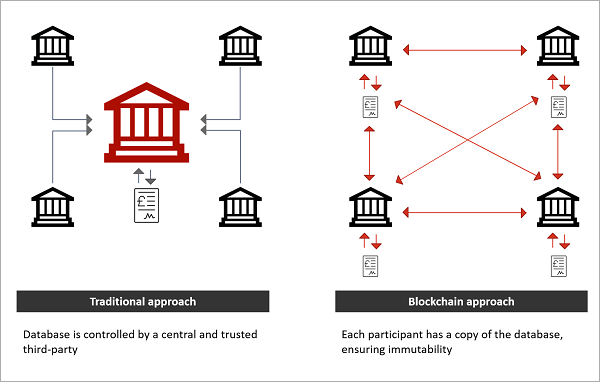
\includegraphics[scale=0.8]{gfx/centralization_vs_decentralization.png}
  \caption{Traditional database vs blockchain approach}
  \label{fig:CentralizedvsDecentralized}
\end{figure}

Returning to the Bitcoin concept, at the beginning, the terms Bitcoin and blockchain were sometimes interchanged, as these words were used to refer: the technology, the protocol for making transactions and the cryptocurrency (money). Therefore, before starting there is one statement that needs to be clear: Bitcoin is a cryptocurrency that uses the blockchain technology. Hence, Bitcoin is just one of the multiple applications that use blockchain. 

However as cryptocurrencies were its first application, we will start explaining what cryptocurrencies are, followed by an explanation of the architectural design of the Bitcoin idea along with its implications.

\subsection{Blockchain 1.0: Cryptocurrencies}

At of the end of January 2018, Coinmarketcap, a cryptocurrency market tracker, lists more than 1,400 cryptocurrencies with an aggregate value approaching USD 700bn.  But what are cryptocurrencies? Cryptocurrencies are a variety of digital currencies pretending to work as a medium of exchange, such as Euro or USD do. As the name suggests, cryptocurrencies apart from being a virtual currency, use cryptography to secure and verify its transactions. The main difference with traditional currencies is that they do not have any physical equivalent in the real world. Nevertheless, they can be used to pay for goods and service, with the advantage of not having any geographical or political borders. For example, GMO Internet, a Japanese company, will start paying parts of employees salaries in cryptocurrencies (Bitcoin).

In this paper, we will set aside whether they can become true currencies or not, and also its political, social or economic impact. The only focus will be the technology behind it, as blockchain can be extended to much more than digital currencies. Thus, we will start from the genesis of the technology, with Bitcoin as its revolutionary innovator.


\subsubsection{Bitcoin}

Bitcoin took the world by surprise in 2009, after Satoshi Nakotomo's white paper publication \cite{nakamoto2008bitcoin} and later its software release. Bitcoin is a cryptocurrency used for making secure transactions across a peer-to-peer (P2P) network. In addition, Bitcoin uses its own protocol that operates in an overlay network, the blockchain. An overlay network is a computer network build in the top of another network, in this case above Internet application's layer.

Furthermore, in Bitcoin, each user possesses a digital Wallet, which is a software program used for performing the transactions. Each of these users is identified by a single public address, composed of 26-35 alphanumeric characters, which is the hash of the user's public key. For example, if user A wants to send Bitcoins to user B, it needs B public address, e.g: 1BvBMSEYstWetqTFn5Au4m4GFg7xJaNVN2. Then, user A creates a message (transaction), attaching receiver's public key with the transferred amount of Bitcoins. This message is signed by sender's private key and sent to the blockchain. Transactions examples can be found in \footnote{\url{https://blockexplorer.com/}}.

From another point of view, the Bitcoin ledger can be interpreted as a state transition system, where there is an initial state, which after a transition function (money transfer), results in a new state. Imagine the last example where A wants to send X to B. The first state is A and B current balance and the transition function will take X from A and insert it to B's account, generating a new state. But what happens if A sends exactly the same payment to two different addresses (B and C) at the same time? This scenario is the so-called double spending attack and consequently, a transaction always needs to be verified by miners in the blockchain before being confirmed.

And how all these miners cooperate efficiently? The answer to this question is one of the most remarkable key factors of Satoshi innovation, which consists of the communication between nodes through a simple decentralized consensus protocol. This consensus protocol consists of multiple algorithms (e.g. Proof of Work), used by specific peers in the Bitcoin network. These peers, also called miners, are responsible for monitoring and verifying all the transactions between users.

\paragraph{Mining}

Bitcoin needs to combine the state transition system with a consensus protocol, to synchronize the order of all transactions among the users.
New transactions are stored in the last block of the blockchain, and a new block is mined every ten minutes. Over time, this creates an ever-growing chain of blocks, which are constantly updated. Thus the name: blockchain. Additionally, a complete history of the transactions is kept, so everyone can verify the last money movements. For instance, a blockchain can be compared to an endless domino game, where all the pieces are placed in vertical one after the other. Each of these pieces references a block, and if one block is not placed correctly (block's error), all the subsequent ones will be affected. Therefore, miner's task is not simple and requires computational power.

\begin{figure}
  \centering
  	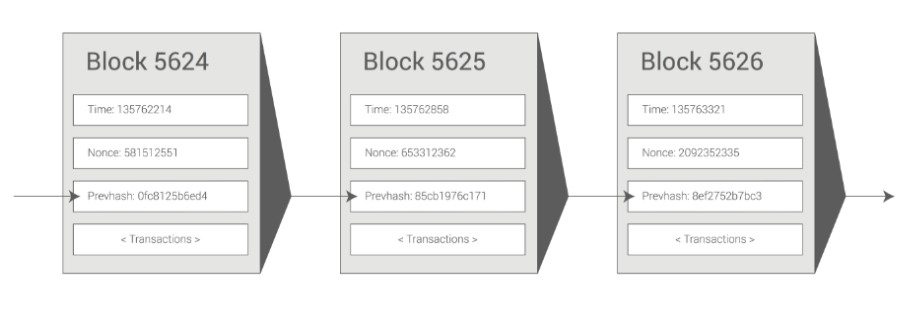
\includegraphics[scale=0.5]{gfx/mining.png}
  \caption{Bitcoin Mining}
  \label{fig:Bitcoin mining}
\end{figure}

Figure \ref{fig:Bitcoin mining} shows a chain of blocks, where each block contains a timestamp, a nonce, a hash reference to the previous block and a list of all the transactions that have been created since the previous block. Thus, for a block being valid needs to satisfy the following requirements: 1. Previous block referenced exists. 2. Block's timestamp is greater than previous block one. 3. Proof-of-work in this block is valid. 4. If any transaction from the transaction lists returns an error, exit. 5. If all previous steps confirmed, store state at the end of the block and return true.

In the third step of the block validation process, appears the term Proof-of-work. Bitcoin uses the Hashcash proof of work algorithm to prove that a block miner spent some computational time creating a block. In particular, the algorithm works with cryptographic hashes, such as SHA1 or SHA256. Proof-of-work is also used in other contexts, such as limiting email spam or denial-of-service attacks (DoS). This technique can lead to a low probability so that the only way to create a valid block is simply trial and error until a valid Proof-of-Work is generated.

Nevertheless, as miners must perform a high computational work, they receive a reward for the mining process. Additionally, if any transaction has a positive balance at the end, it is also destinated to the miner.

\paragraph{Merkle Trees}


\subsection{Blockchain 2.0: Smart contracts}

 In this second part, the Ethereum blockchain will be compared with the 1st generation one, followed by the discussion of concepts, such as smart contracts or decentralized applications.
 
\subsubsection{Ethereum}

First Bitcoin vs Ethereum Blockchain

Ether = gas price x gas amount + value.

\subsection{Blockchain types}


\subsection{Decentralized applications}

Decentralising existing services/ Use cases...

\section{Network Virtualization}

Understanding network virtualization as the customer willingness to embed resources in a virtual network, provided by one or multiple infrastructure providers
\subsection{Multi-Provider Virtual Network Embedding}

\section{Auction Mechanisms}

\subsection{Vickrey Auction Model}

Under the Vickrey auction Model, the VN bidders will quote a price of hosting a virtual resource, and the lowest quote wins the auction, but the service is rendered at the price of the second lowest quote. InP offers prices proportional to the actual cost of the virtual resource (Strategy proof).

Vickrey auction -> Sealed-bid, second-price auction.
Pros and cons Vickrey auction deep research explaining always WHY.

\section{Summary}


%*****************************************
\chapter{Related Work}
\label{ch:relatedwork}
%*****************************************
\hint{This chapter should give a comprehensive overview on the related work done by other authors followed by an analysis why the existing related work is not capable of solving the problem described in the introduction.
The chapter should have a length of about three to five pages!}
\section{Related Work Area 1}

IOTA-TANGLE VS BLOCKCHAIN VS DATABASE

\section{Related Work Area 2}

OTHER PAPERS IN Multi-provider network embedding
\section{Analysis of Related Work}

\section{Summary}

%*****************************************
\chapter{Design}
\label{ch:design}
%*****************************************
\hint{This chapter should describe the design of the own approach on a conceptional level without mentioning the implementation details. The section should have a length of about five pages.}

\section{Requirements and Assumptions}

\section{System Overview}

\subsection{Component 1}

\subsection{Component 2}

\section{Summary}

%*****************************************
\chapter{Implementation}
\label{ch:implementation}
%*****************************************

\hint{This chapter should describe the details of the implementation addressing the following questions: \\ \\
1. What are the design decisions made? \\
2. What is the environment the approach is developed in? \\
3. How are components mapped to classes of the source code? \\
4. How do the components interact with each other?  \\
5. What are limitations of the implementation? \\ \\
The section should have a length of about five pages.}
\section{Design Decisions}

\section{Architecture}

\section{Interaction of Components}

\section{Summary}

%*****************************************
\chapter{Evaluation}
\label{ch:evaluation}
%*****************************************
\hint{This chapter should describe how the evaluation of the implemented mechanism was done. \\ \\
1. Which evaluation method is used and why? Simulations, prototype? \\
2. What is the goal of the evaluation? Comparison? Proof of concept? \\
3. Wich metrics are used for characterizing the performance, costs, fairness, and efficiency of the system?\\
4. What are the parameter settings used in the evaluation and why? If possible always justify why a certain threshold has been chose for a particular parameter.  \\
5. What is the outcome of the evaluation? \\ \\
The section should have a length of about five to ten pages.}
\section{Goal and Methodology}

\section{Evaluation Setup}

\section{Evaluation Results}

\section{Analysis of Results}


%*****************************************
\chapter{Conclusions}
\label{ch:closure}
%*****************************************

\hint{This chapter should summarize the thesis and describe the main contributions of the thesis. Subsequently, it should describe possible future work in the context of the thesis. What are limitations of the developed solutions? Which things can be improved?
The section should have a length of about three pages.}

\section{Summary}

\section{Contributions}

\section{Future Work}

\section{Final Remarks}
